\documentclass[11pt]{article}
\usepackage{amsmath,textcomp,amssymb,geometry,graphicx,enumerate}
\usepackage{algorithm} % Boxes/formatting around algorithms
\usepackage[noend]{algpseudocode} % Algorithms
\usepackage{hyperref}
\usepackage{xcolor}
\usepackage{geometry}
\usepackage{caption}
\hypersetup{
    colorlinks,
    linkcolor={red!50!black},
    citecolor={blue!50!black},
    filecolor=magenta,      
    urlcolor={blue!80!black}
}

\geometry{
    left=40mm,
    right=40mm,
}
\captionsetup{labelfont=bf}
\pagestyle{myheadings}

\title{\textbf{Convolutional Neural Networks for Bone Marrow Edema and Synovitis Segmentation in Rheumatoid Arthritis}}
\date{}
\author{Qitao Li, Xiaojuan Li, Valentina Pedoia}

\begin{document}
\maketitle

\noindent \textbf{Abstract.} Quantifying bone marrow edema (BME) and synovitis legions in Magnetic Resonance (MR) images of patients with Rheumatoid Arthritis (RA) is an important tool for diagnosis and treatment of RA. Manual segmentation of lesions is costly due to both the complex positioning of the lesions and the size of the MR volumes. In this work, we present an automatic segmentation method using a fully-convolutional Convolutional Neural Network (CNN) with an encoder-decoder architecture. The network is trained on $ 128 \times 128 \times 16$ patches sampled from 24 $512 \times 512 \times 20$ MR volumes and outputs a voxel-wise segmentation of the input patch. Furthermore, we train with a loss function based on Dice coefficient to deal with class-imbalance. We find that the network performs with an average dice coefficient of $c$ on a test set. The implementation and code are available at \url{https://github.com/cosmicac/ucsf-mri-seg.} 

\section{Introduction}

Rheumatoid arthritis (RA) is a chronic inflammatory disease affecting 1.3 million Americans that causes destruction of articular and periarticular structures, of which wrist joints may be among the first affected \hyperref[gab]{[1]}. Early diagnosis and monitoring of abnormalities within joint structures are important for successful therapy.

Magnetic Resonance (MR) images of patients' wrists can reveal synovitis and bone marrow edema (BME) lesions. The Outcome Measures in Rheumatology Clinical Trials (OMERACT) has developed a RA MRI Scoring (RAMRIS) system to assess these lesions in a reliable and reproducible manner. However, because RAMRIS does not use the direct volumes of the lesions but instead uses a discrete score to measure the severity of lesions, it is a semi-quantitative system that can result in considerable inter-reader variability \hyperref[hodge]{[2]}. Using the true volume of lesions would offer a more objective measurement of disease progression. 

Manual delineation of lesions is a time-consuming and tricky task that requires a skilled operator. Comparison between multiple MR sequences is often neccessary. Moreover, an operator must take into consideration the three spatial dimensions of the MR volume while working through the volume one 2D slice at a time. Semi-automatic methods that combine rough manual outlining with thresholding can help speed up the process, but the choice of thresholding level can introduce biases and inaccuracies. A fuly-automatic, fast segmentation method that utilizes the information of 3 spatial dimensions of the MR volumes to segment synovitis and BME lesions would be desirable.

A method for automatic segmentation of synovitis in the wrist was proposed by Czaplicka et al., but it relies on complex, less generalizable wrist-bone segmentation and thresholding \hyperref[cza]{[3]}. In recent years, convolutional neural networks (CNNs) have been used in image classification and segmentation contexts to great success due to their ability to extract and learn heirarchical features. CNNs first achieved acclaim in their abilities to classify whole images as demonstrated by Krizhevsky et al. \hyperref[kriz]{[4]}. However, a segmentation context requires pixel-wise classification instead of whole-image classification. Long et al. addressed this with a fully-convolutional architecture that outputs dense pixel-wise predictions \hyperref[long]{[5]}. A recent, popular innovation to the fully-convolutional architecture that has produced great restuls is the "deconvolutional", or "encoder-decoder" architecture \hyperref[noh]{[6,7,8]}. This architecture features a symmetrical network that first learns an encoding by downsampling with convolutions and then learns to decode into a segmentation mask by upsampling with "deconvolutions". 

In this work, we present a CNN with a 3D encoder-decoder architecture to automatically segment synovitis and BME lesions in MR volumes. Similar to V-Net from Milletari et al., we equip our network with a loss function based on the Dice coefficient to deal with class-imbalance \hyperref[vnet]{[8]}. We show that our CNN can perform fast and accurately on test patients. 

\section{Materials}

Our dataset consists of 32 MRI volumes of dimension $512 \times 512 \times 20$ from 16 patients at various timepoints. These volumes are available in 3 sequences: a T1-weighted pre-gadolinium injection sequence, a T1-weighted post-gadolinium injection sequence, and T2-weighted sequence. The two T1-weighted sequences form the two input channels for our synovitis segmentation network, while the T2-weighted sequence forms the input channel for our BME segmentation network. We split up our dataset into 24 volumes for the training set and 8 volumes for a validation set. 

\section{Method}
\begin{figure}
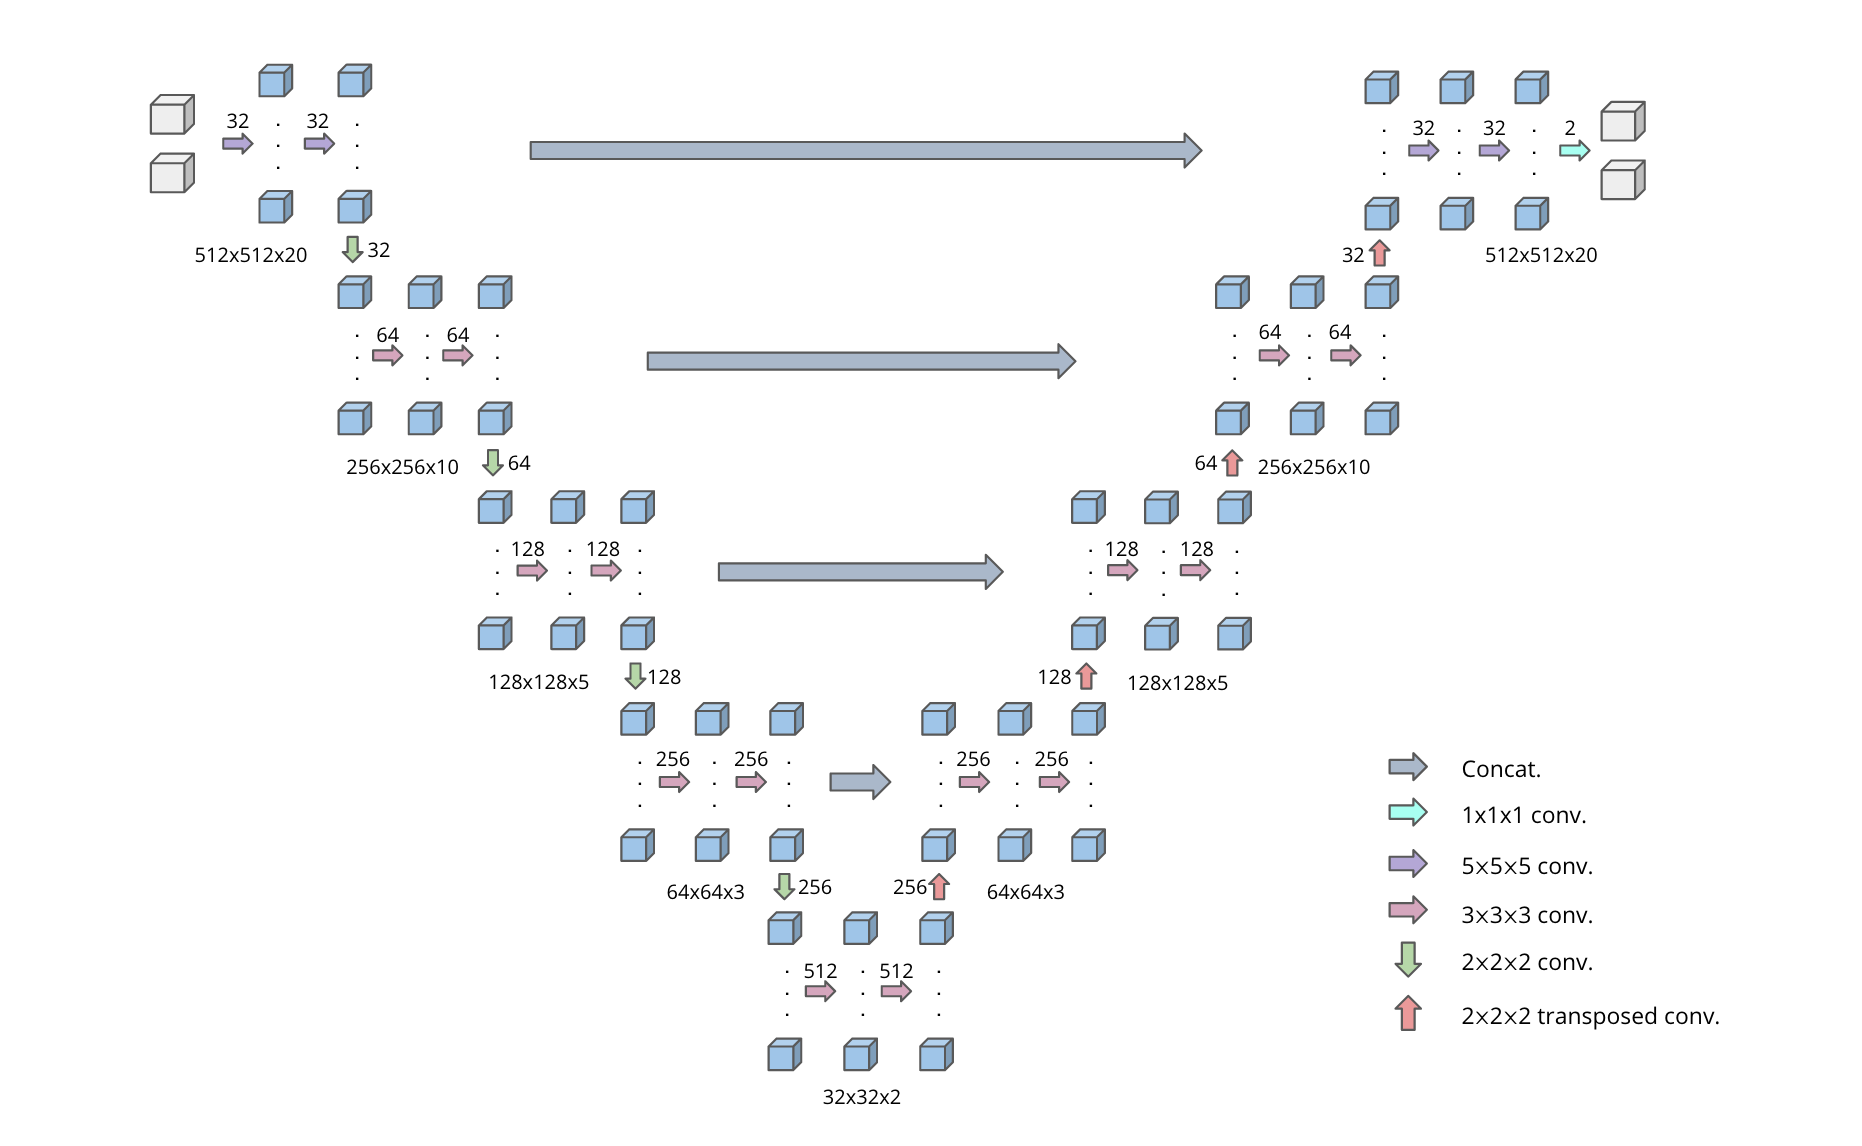
\includegraphics[width=\textwidth]{figures/fig2.png}
\caption{The architecture of our CNN. The numbers on top of the arrows are the number of filters. The spatial dimensions of each level of the CNN are on below.}
\end{figure}

\subsection{Architecture}
Figure 1 gives a visual representation of our network architecture. The left half of the network is downsampling to learn an encoding, while the right half of the network decodes the learned encoding and outputs a segmentation mask at the end.

The network consists of four layers in terms of spatial dimensions, each one half the size of the previous layer. Each layer consists of two convolutional layers. Convolutions within layers have stride of 1 and are padded to preserve the same dimensions. On the left side of the network, $2 \times 2 \times 2$ convolutions with stride 2 are are used to downsample between layers, whereas on the right side, $2 \times 2 \times 2$ transposed convolutions with stride 2 are used to learn an upsampling. In the first layer, the kernel size of the convolutions is $5 \times 5 \times 5$ in order to capture more complex features on the lowest level of th e heirarchy of features. Within all the other layers, kernels of size $3 \times 3 \times 3$ are employed. All convolutional layers are equipped with ReLU non-linearities.

As with a standard CNN, the receptive field of filters in consecutive layers is increased linearly within layers, and doubled when moving down a layer. Since the spatial dimensions are halved when moving down a layer, we can double the number of filters. Likewise, the spatial dimensions are doubled when moving up a layer so the number of filters is halved.   

Learning an upsampling or interpolation scheme on the right side of the network can result in coarseoutlines and segmentations due to loss of detailed information on the left side encoding path. To help deal with this, we employ fine grained feature forwarding from each level on the left side to the corresponding level on the right side, like many previous works \hyperref[noh]{[5,6,7,8]}. This allows for a more precise upsampling to be learned from the transposed convolutions. 

In the final convolutional layer on the right side, we employ a two filters with kernel size of $1 \times 1 \times 1$ in order to output our two volumes of logits, each with the same spatial dimension as the input ($128 \times 128 \times 16$), one for each class. These logits are then passed to a softmax operation to extract our final class probabilities for each voxel. 

\subsection{Training}

We train with a loss function based on Dice coefficient as follows, where $P$ is the length $N$ ($N = 128 \times 128 \times 16$) vector of predicted probabilites (output of softmax), $Y$ is the length $N$ vector of binary ground truth labels, and $\gamma$ is a small smoothing factor:

\begin{align*}
D = \frac{2\sum_{i}^{N}p_iy_i + \gamma}{\sum_{i}^{N}p_i + \sum_{i}^{N}y_i + \gamma}
\end{align*}

Note that $p_i \in P$ are the raw probabilities and not the binary predictions that would be used to calculate the Dice coefficient when evaluating accuracy - this is because a non-differentiable $argmax$ operation would be neccessary to extract the predictions from the probabilities, which would prevent gradient calculation by the optimizer. 

We train using the Adam optimizer with initial learning rate $\alpha = 1e-03$, $\beta_1 = 0.9$, $\beta_2 = 0.999$, and $epsilon =1e-04$. We use batch size of $8$ and decay the learning rate by a factor of $0.25$ every $10$ epochs. 

\section{Results}
\section{Conclusion}

\newpage
\section*{References}
\begin{enumerate}

\item \label{gab} Gabriel S.E., The epidemiology of rheumatoid arthritis, Rheum. Dis. Clin. North
Am. 27 (2001) 269–281.

\item \label{hodge} Hodgson R.J., O'Connor P., Moots R. MRI of rheumatoid arthritis - image quantitation for the assessment of disease actiivty, progression and response to therapy. Rheumatology 47 (2008) 13-21. 

\item \label{cza} Czaplicka K, Wojciechowski W, Wlodarczyk J, Urbanik A, Tabor Z. Automated assessment of synovitis in 0.2 T magnetic resonance images of the wrist. Computers in Biology and Medicine 67 (2015) 116-125. 

\item \label{kriz} Krizhesky A, Sutskever I, Hinton G.E. ImageNet classification with deep convolutional neural networks. NIPS (2012) 1106-1114. 

\item \label{long} Long J, Shelhamer E, Darrell T. Fully convolutional networks for semantic segmentation (2014). arXiv:1411.4038 [cs.CV]

\item \label{noh} Noh H, Hong S, Han B. Learning deconvolution network for semantic segmentaiton. Proceedings of the IEEE International Conference on Computer Vision (2015) 1520-1528.

\item \label{unet} Ronneberger O, Fischer P, Brox T. U-net: Convolutional networks for biomedical image segmentation. Medical Image Computing and Computer-Assisted Intervention - MICCAI 2015 (2015) 234-241.

\item \label{vnet} Milletari F, Navab N, Ahmadi S. V-Net: Fully Convolutional Neural Networks for Volumetric Medical Image Segmentation (2016). arXiV:1606.04797 [cs.CV] 
\end{enumerate}

\end{document}
